\chapter{Appendices}\label{ch:appendicies}
\section{Appendix A - Additional Fine-Tuning Results}\label{sec:appA}
\begin{figure}[h!]
    \centering
    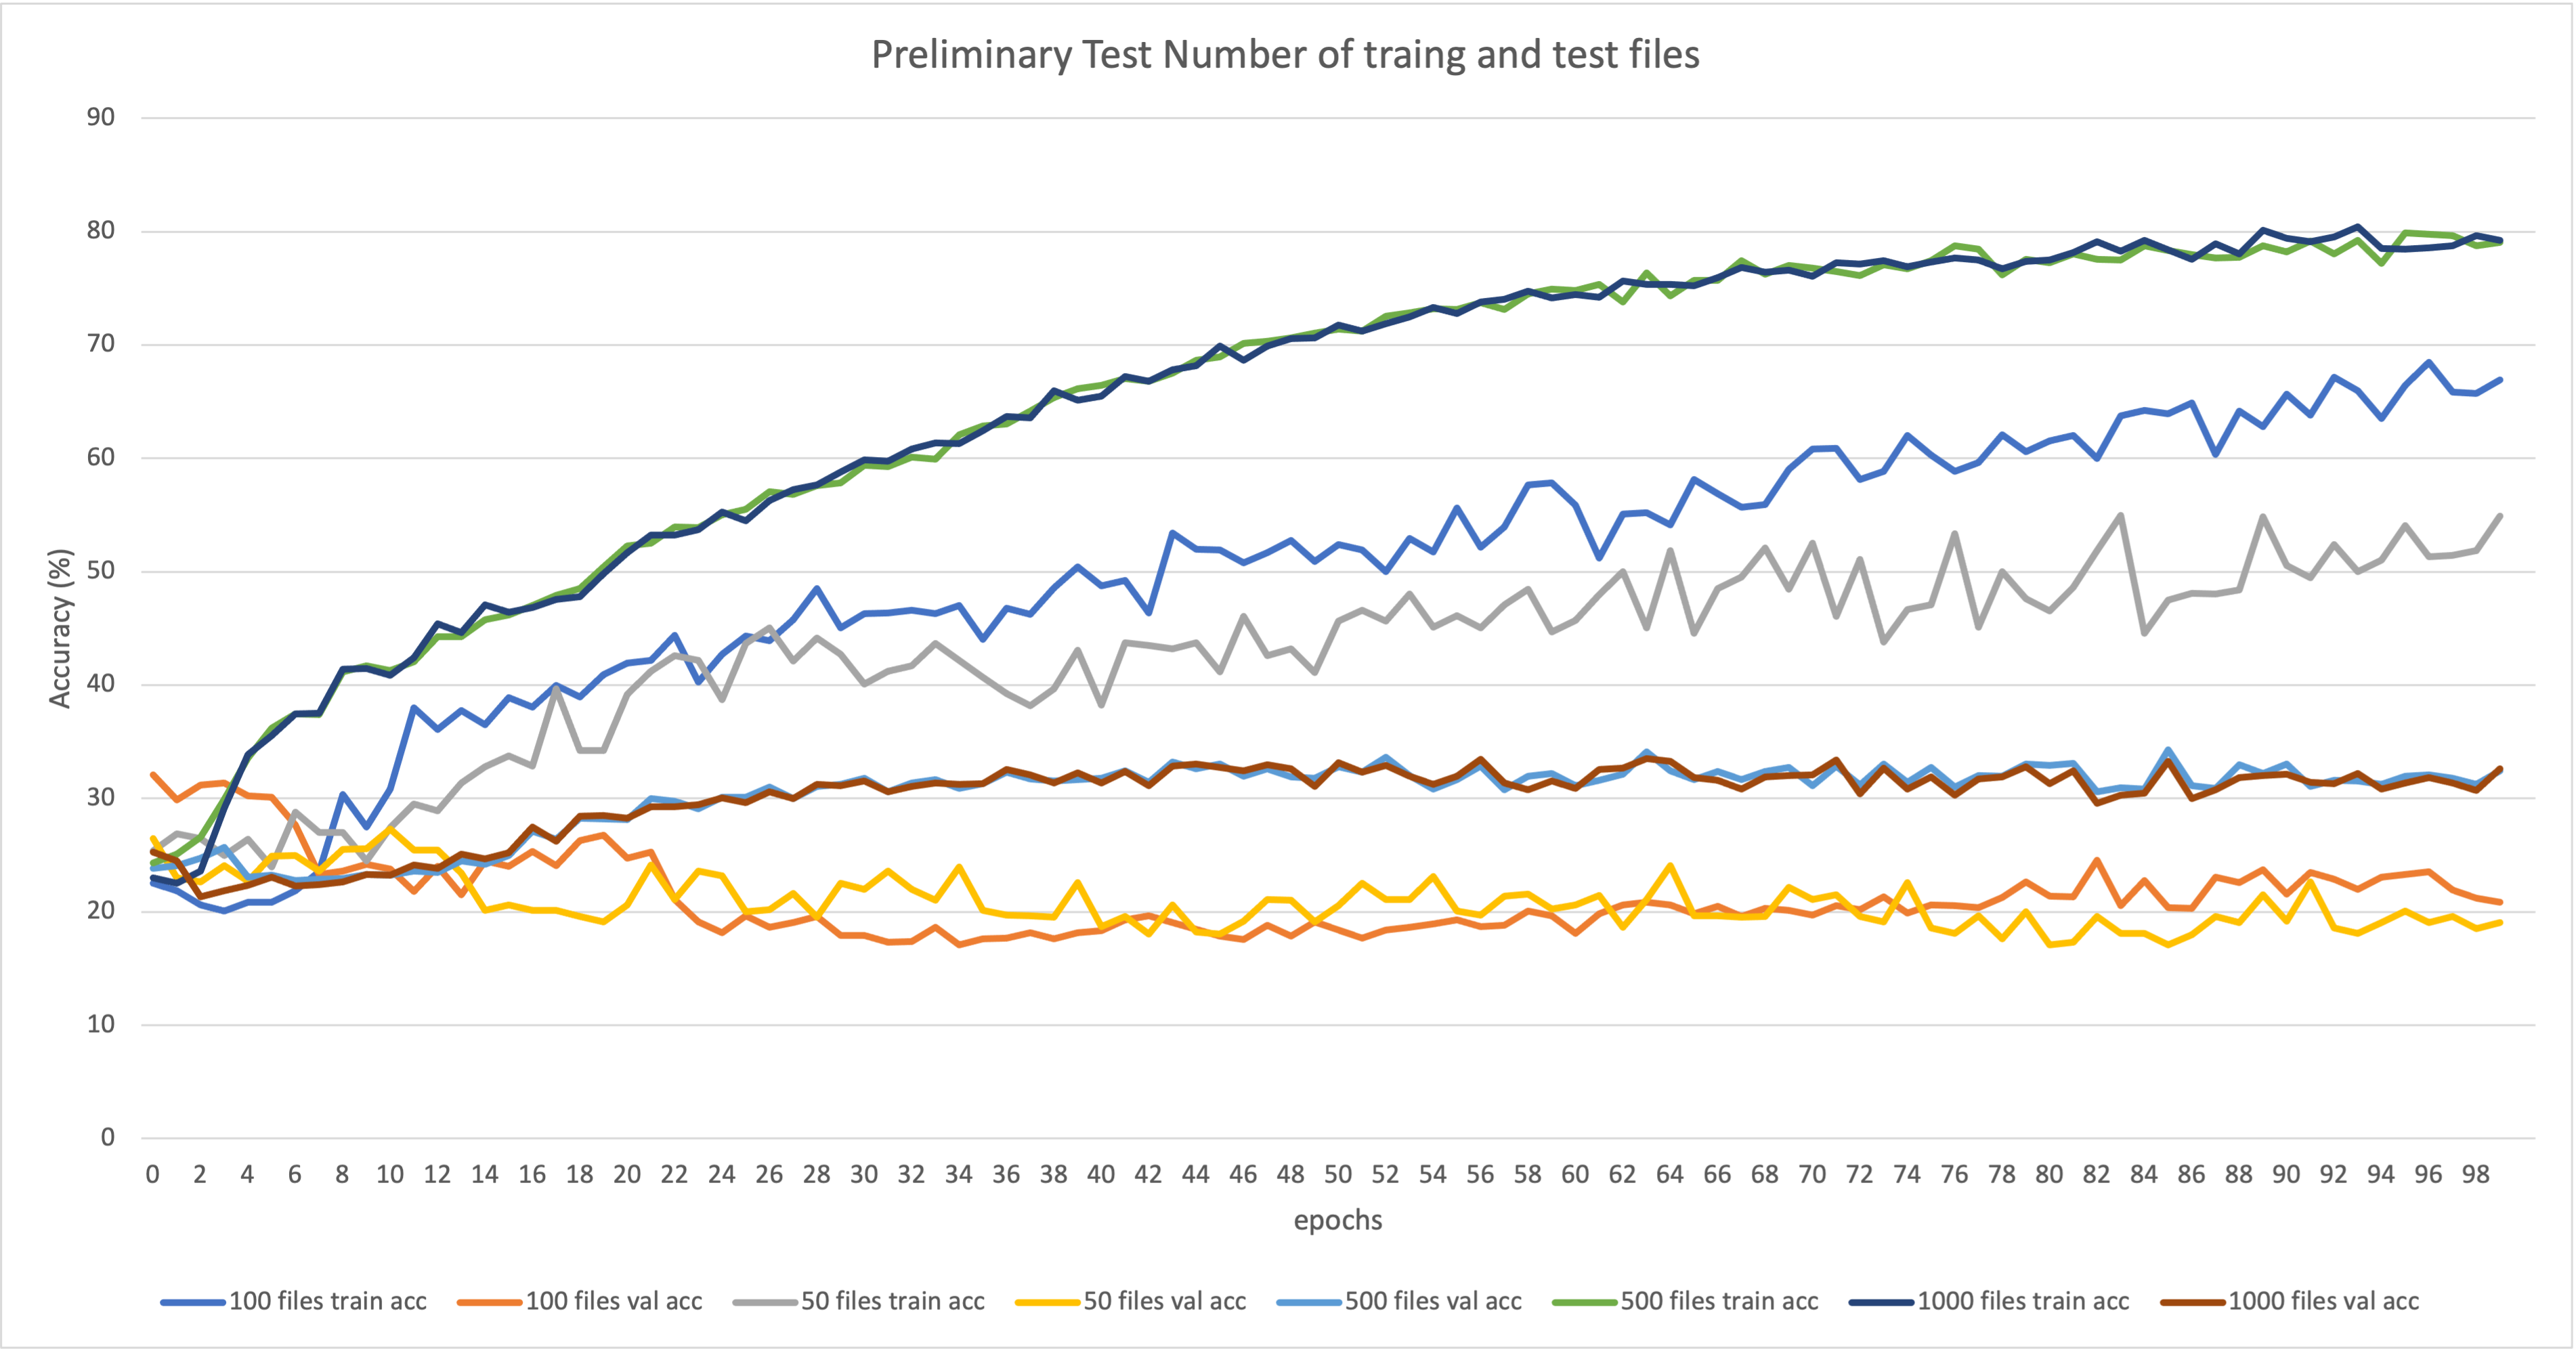
\includegraphics[width=\textwidth]{appendix/prelimNumFiles.png}
    \caption{Preliminary Testing Number of Files.}
\end{figure}

\begin{figure}[h!]
    \centering
    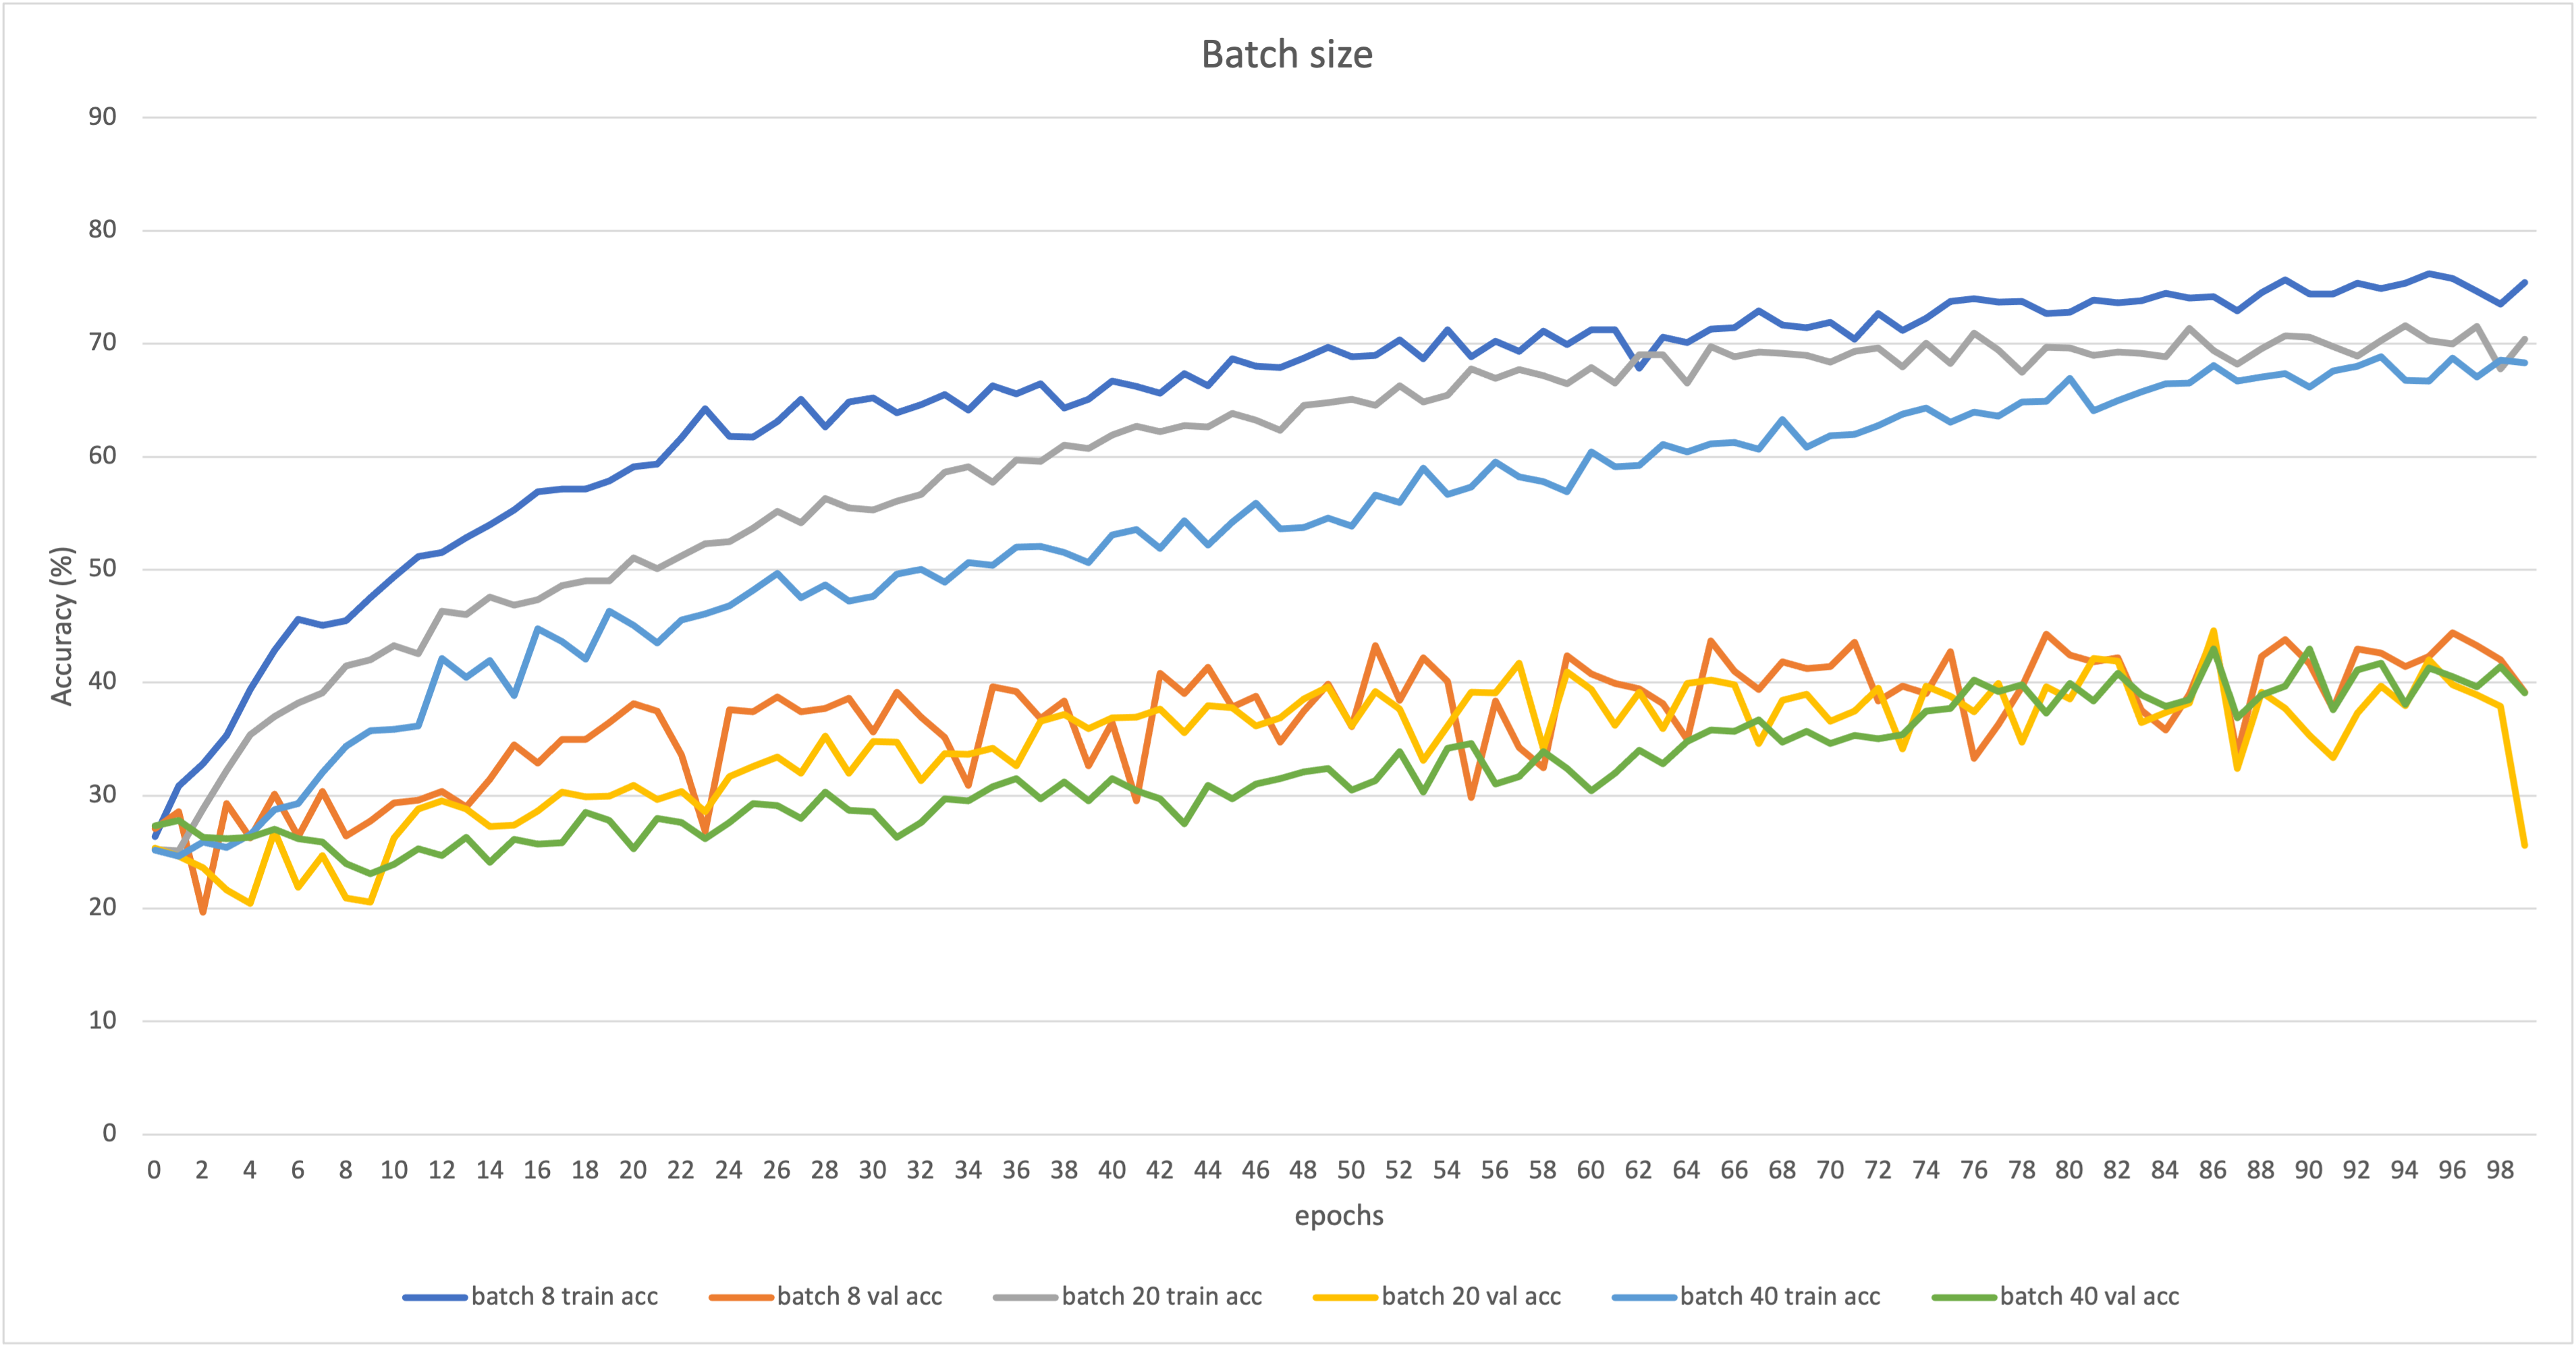
\includegraphics[width=\textwidth]{appendix/batch.png}
    \caption{Preliminary Testing Batch Size.}
\end{figure}

\begin{figure}[h!]
    \CommonHeightRow{
        \begin{floatrow}[2]
            \ffigbox[\FBwidth]
            {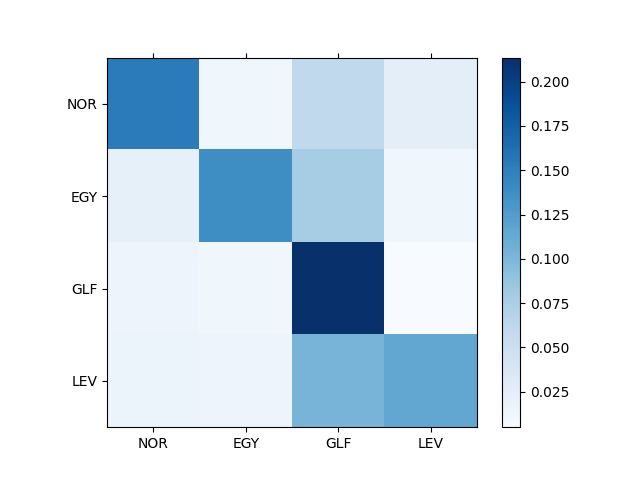
\includegraphics[height=6cm]{appendix/ADI17-hubert-norm.png}}
            {\caption{Hubert \newline Normalised Confusion  Matrix Colour Map.}}
            \ffigbox[\FBwidth]
            {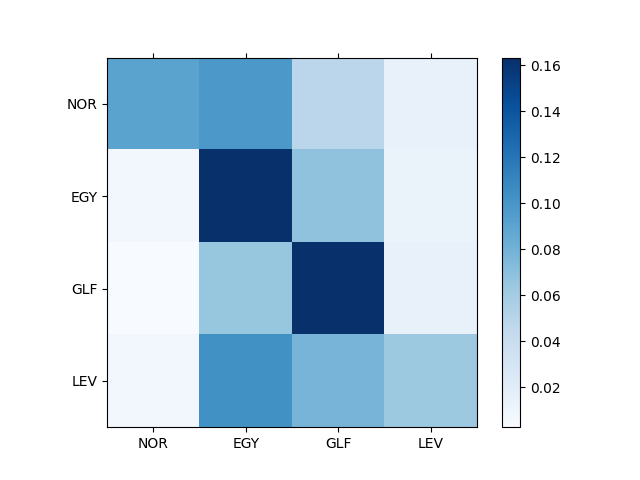
\includegraphics[height=6cm]{appendix/ADI17-w2v2-base-norm.png}}
            {\caption{Wav2vec 2.0 Base \newline Normalised Confusion Matrix Colour Map.}}
        \end{floatrow}}
\end{figure}

\begin{figure}[h!]
    \CommonHeightRow{
        \begin{floatrow}[2]
            \ffigbox[\FBwidth]
            {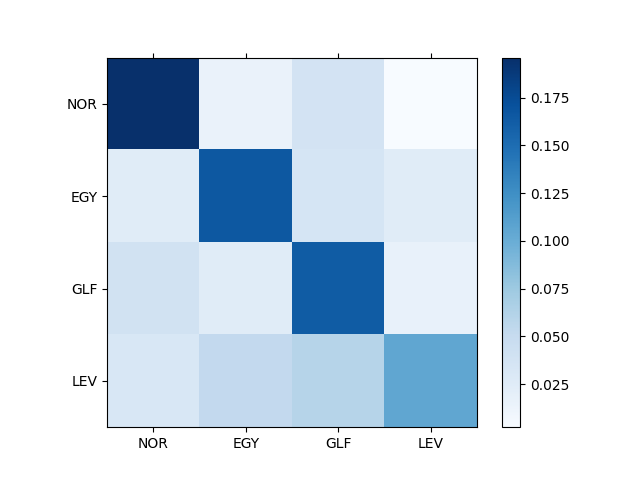
\includegraphics[height=6cm]{appendix/ADI17-xlsr-w2vsid2-norm.png}}
            {\caption{Wav2vec SID \newline Normalised Confusion  Matrix Colour Map.}}
            \ffigbox[\FBwidth]
            {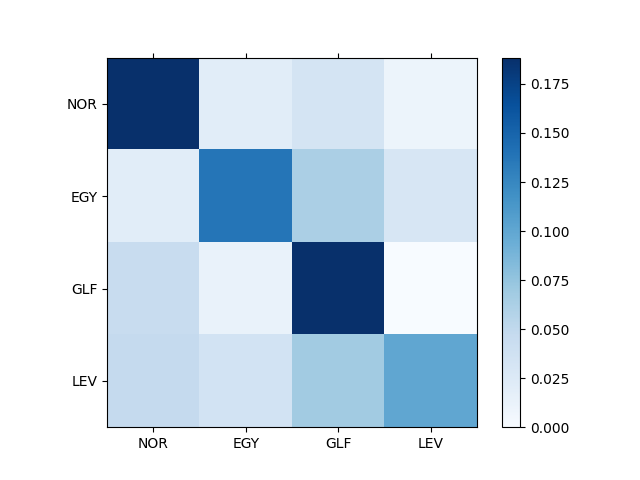
\includegraphics[height=6cm]{appendix/ADI17-lid2-norm.png}}
            {\caption{Wav2vec LID \newline Normalised Confusion Matrix Colour Map.}}
        \end{floatrow}}
\end{figure}

\begin{figure}[h!]
    \CommonHeightRow{
        \begin{floatrow}[2]
            \ffigbox[\FBwidth]
            {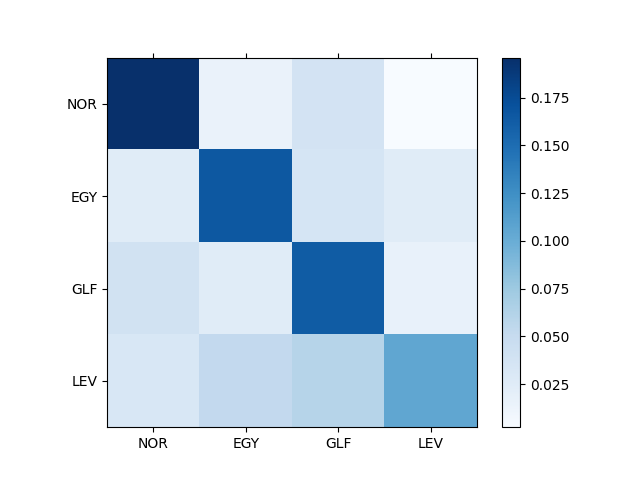
\includegraphics[height=6cm]{appendix/ADI17-xlsr-w2vsid2-norm.png}}
            {\caption{Wav2vec SID \newline Normalised Confusion  Matrix Colour Map.}}
            \ffigbox[\FBwidth]
            {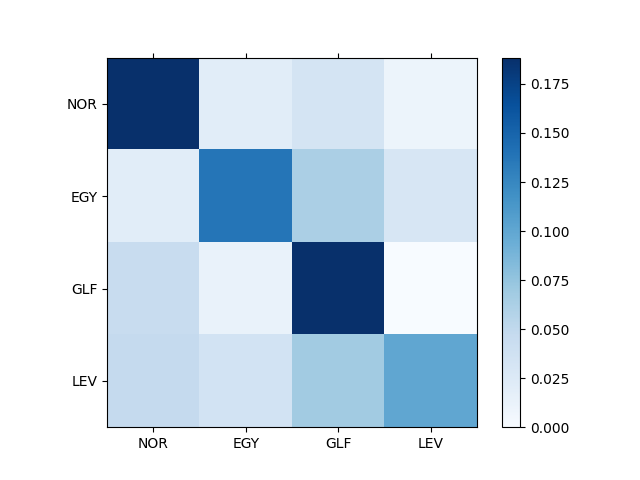
\includegraphics[height=6cm]{appendix/ADI17-lid2-norm.png}}
            {\caption{Wav2vec LID \newline Normalised Confusion Matrix Colour Map.}}
        \end{floatrow}}
\end{figure}

\begin{figure}[h!]
    \CommonHeightRow{
        \begin{floatrow}[2]
            \ffigbox[\FBwidth]
            {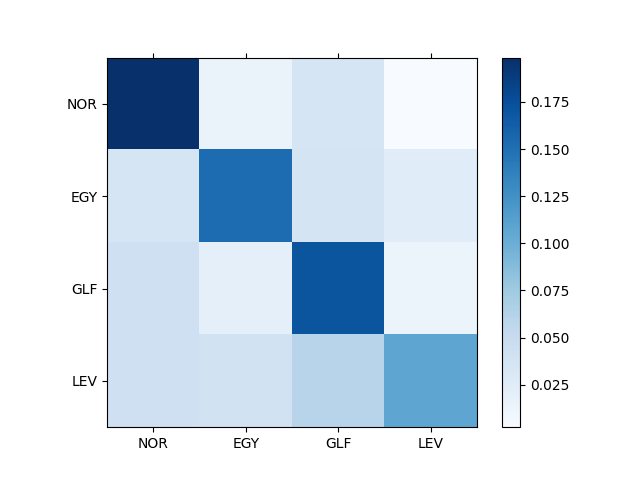
\includegraphics[height=6cm]{appendix/ADI17-xlsr-arabic-norm.png}}
            {\caption{XLSR Arabic \newline Normalised Confusion  Matrix Colour Map.}}
            \ffigbox[\FBwidth]
            {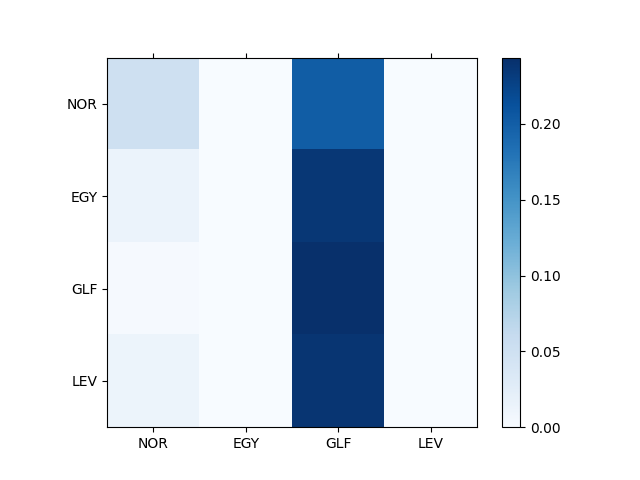
\includegraphics[height=6cm]{appendix/ADI17-xlsr-basic-norm.png}}
            {\caption{XLSR \newline Normalised Confusion Matrix Colour Map.}}
        \end{floatrow}}
\end{figure}


\begin{figure}[h!]
    \CommonHeightRow{
        \begin{floatrow}[2]
            \ffigbox[\FBwidth]
            {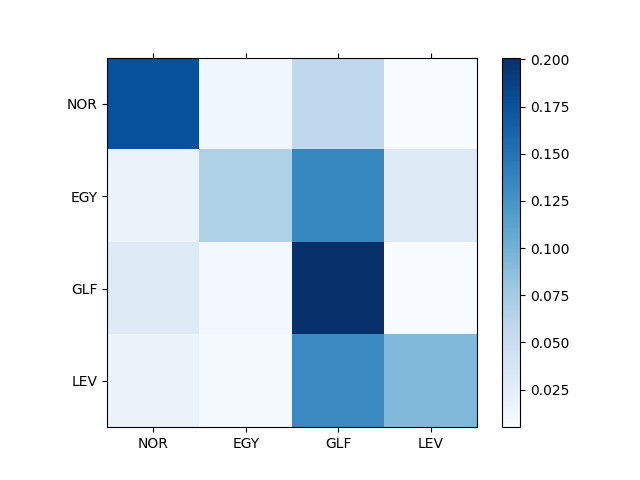
\includegraphics[height=6cm]{appendix/ADI17-xlsr-dnn-norm.png}}
            {\caption{DNN 3 layer \newline Normalised Confusion  Matrix Colour Map.}}
            \ffigbox[\FBwidth]
            {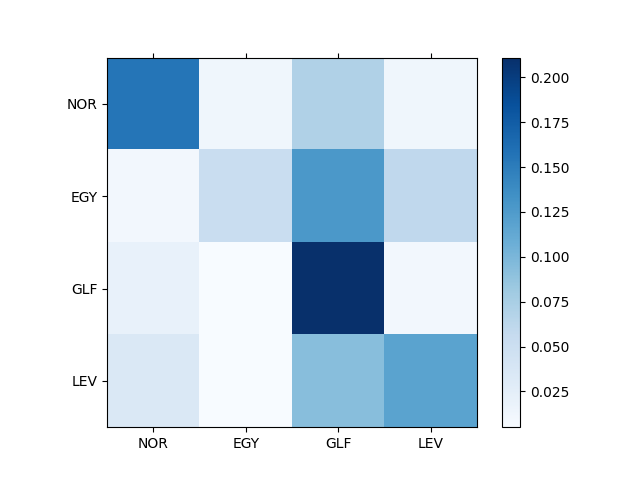
\includegraphics[height=6cm]{appendix/ADI17-xlsr-dnn-4layer-norm.png}}
            {\caption{DNN 4 layer \newline Normalised Confusion Matrix Colour Map.}}
        \end{floatrow}}
\end{figure}

\begin{figure}[h!]
    \CommonHeightRow{
        \begin{floatrow}[2]
            \ffigbox[\FBwidth]
            {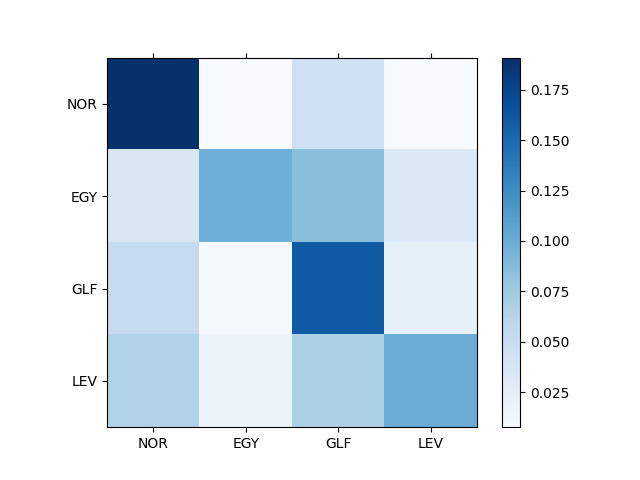
\includegraphics[height=6cm]{appendix/ADI17-xlsr-dnn_6layer-norm.png}}
            {\caption{DNN 6 layer \newline Normalised Confusion  Matrix Colour Map.}}
            \ffigbox[\FBwidth]
            {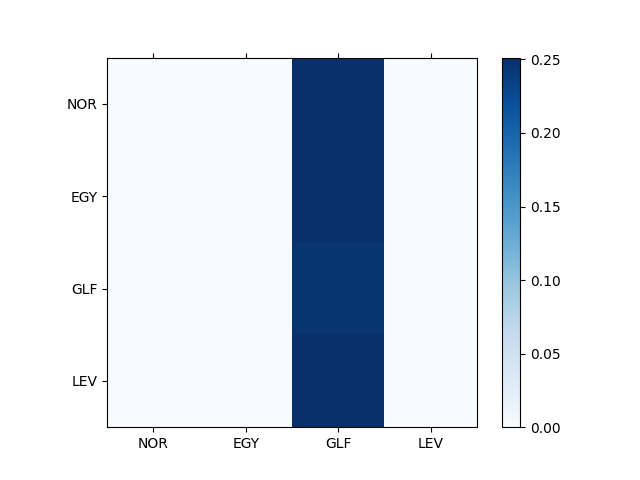
\includegraphics[height=6cm]{appendix/ADI17-xlsr-lstm-norm.png}}
            {\caption{LSTM \newline Normalised Confusion Matrix Colour Map.}}
        \end{floatrow}}
\end{figure}

\begin{figure}[h!]
    \centering
    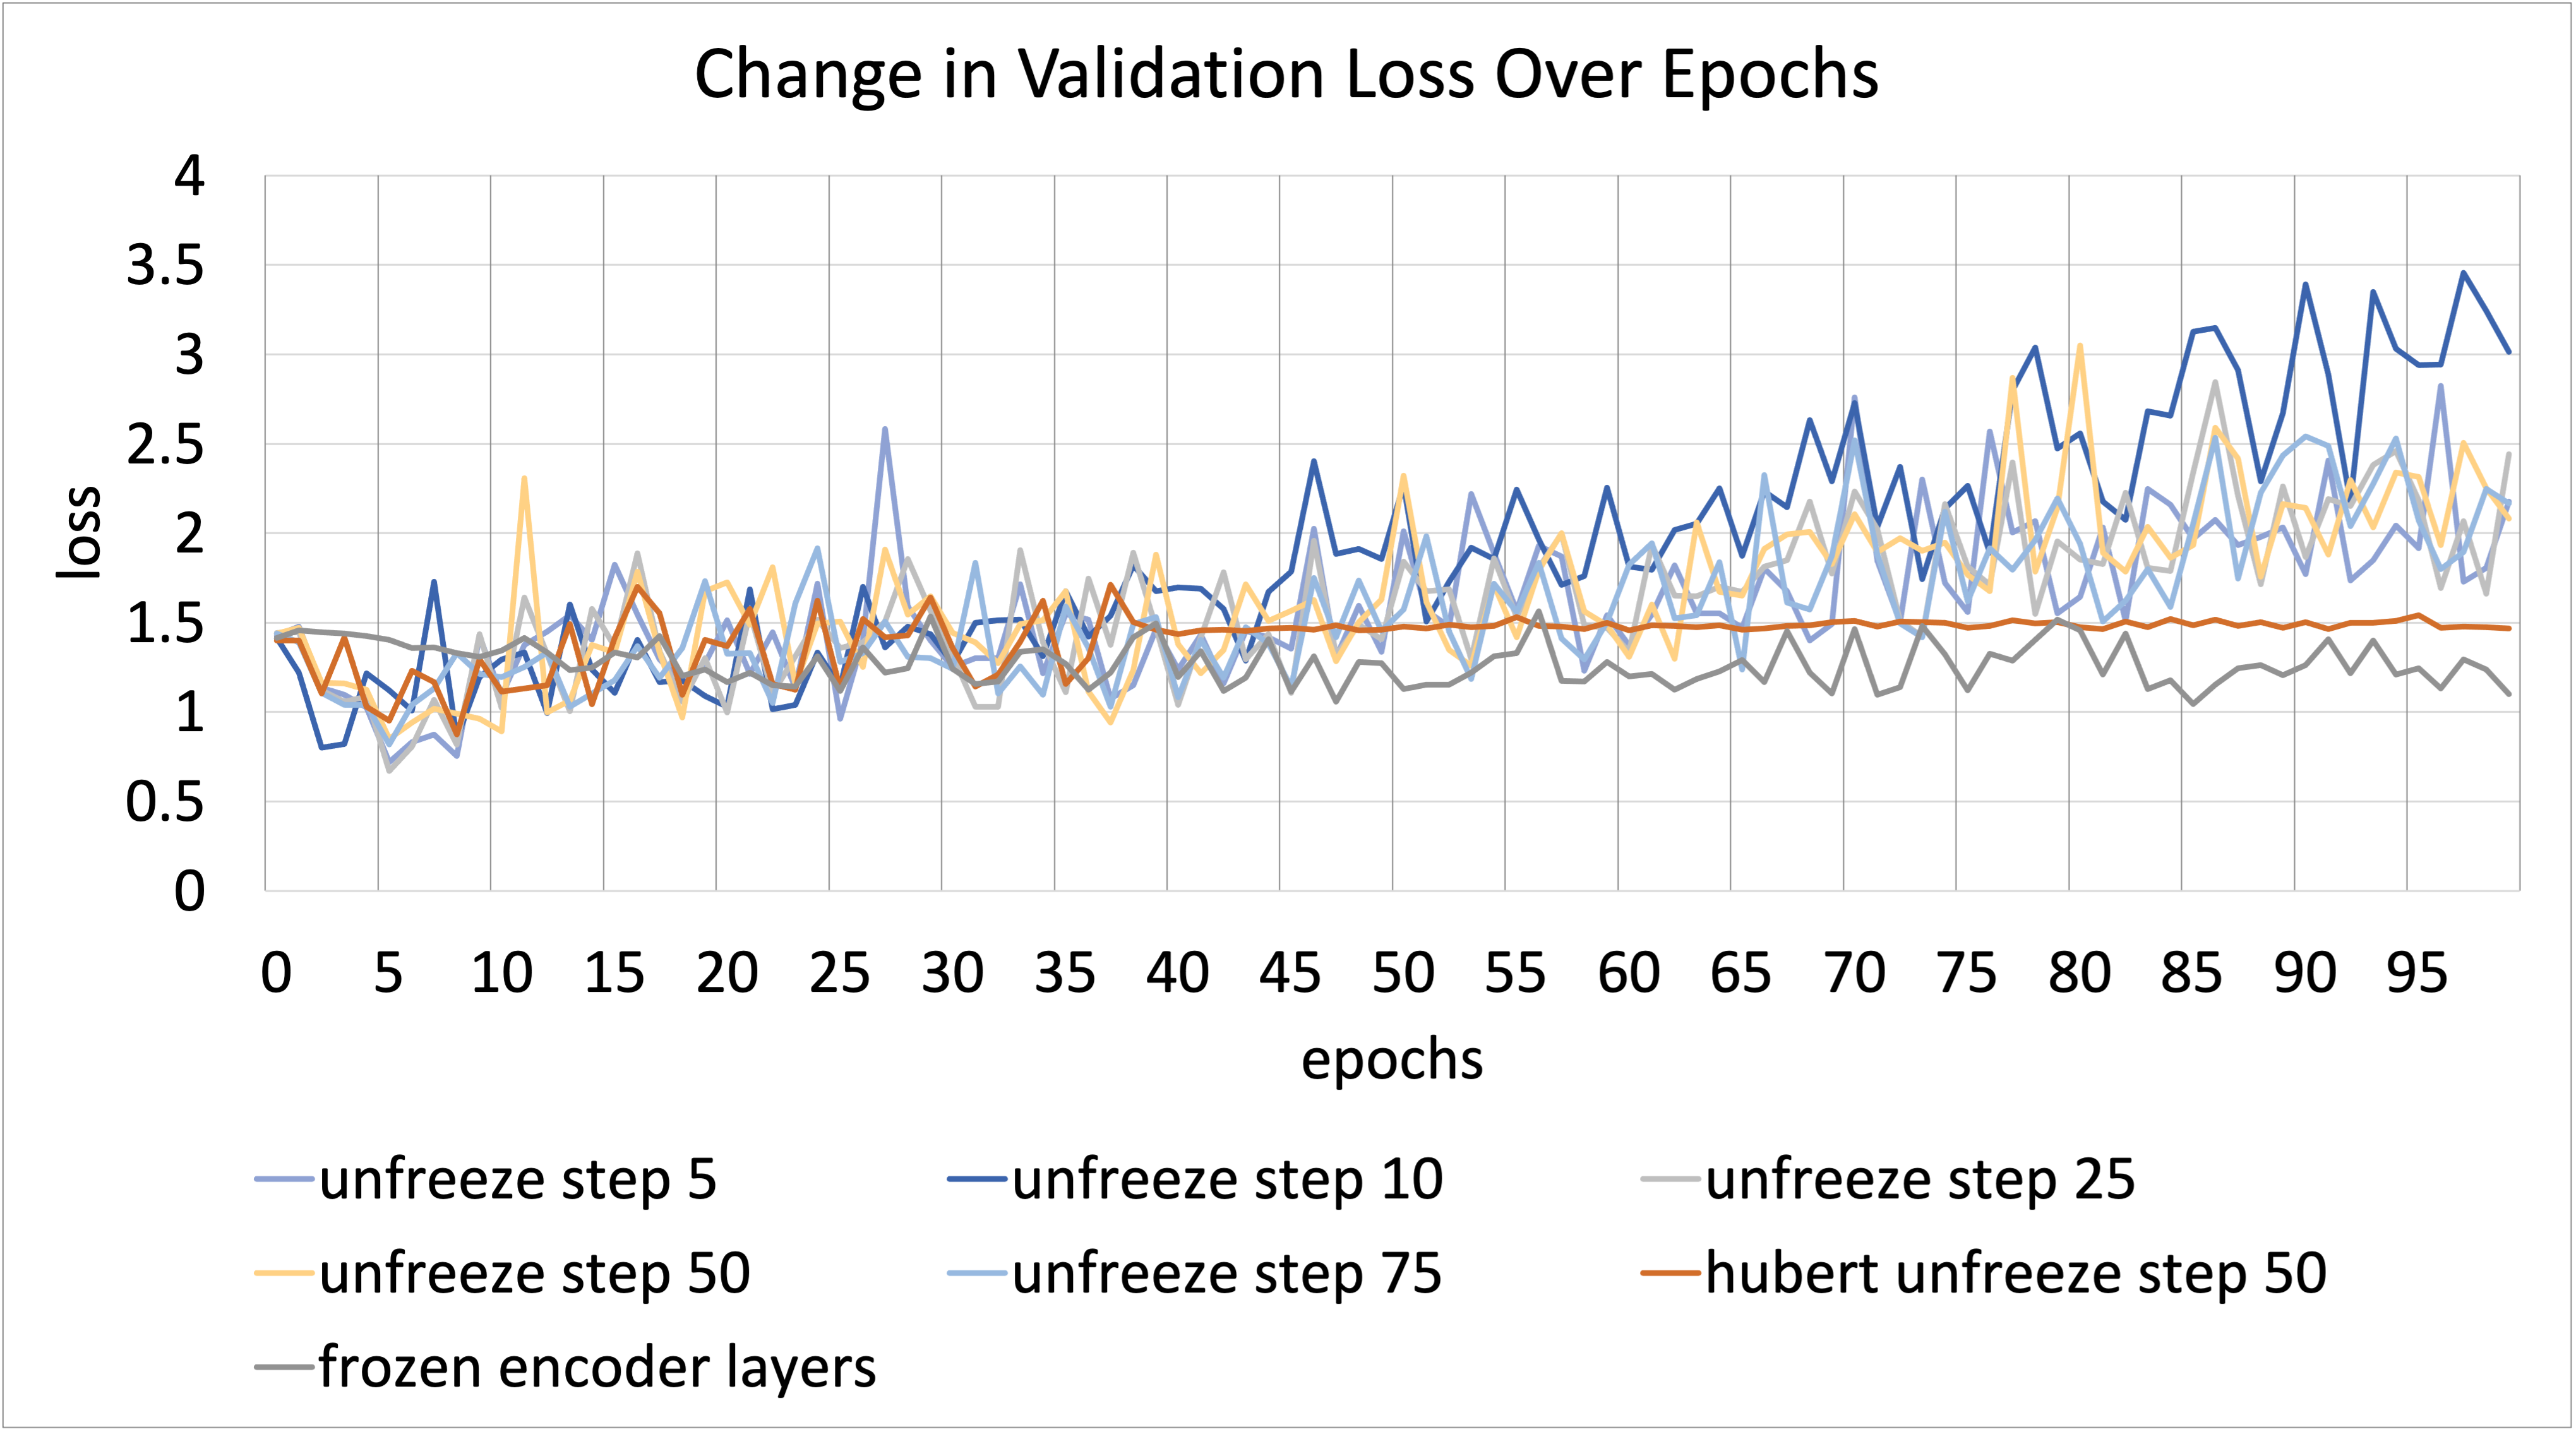
\includegraphics[width=\textwidth]{appendix/UnfreezeLoss.png}
    \caption{Unfreezing encoder layers change in validation loss.}
\end{figure}

\begin{figure}[h!]
    \centering
    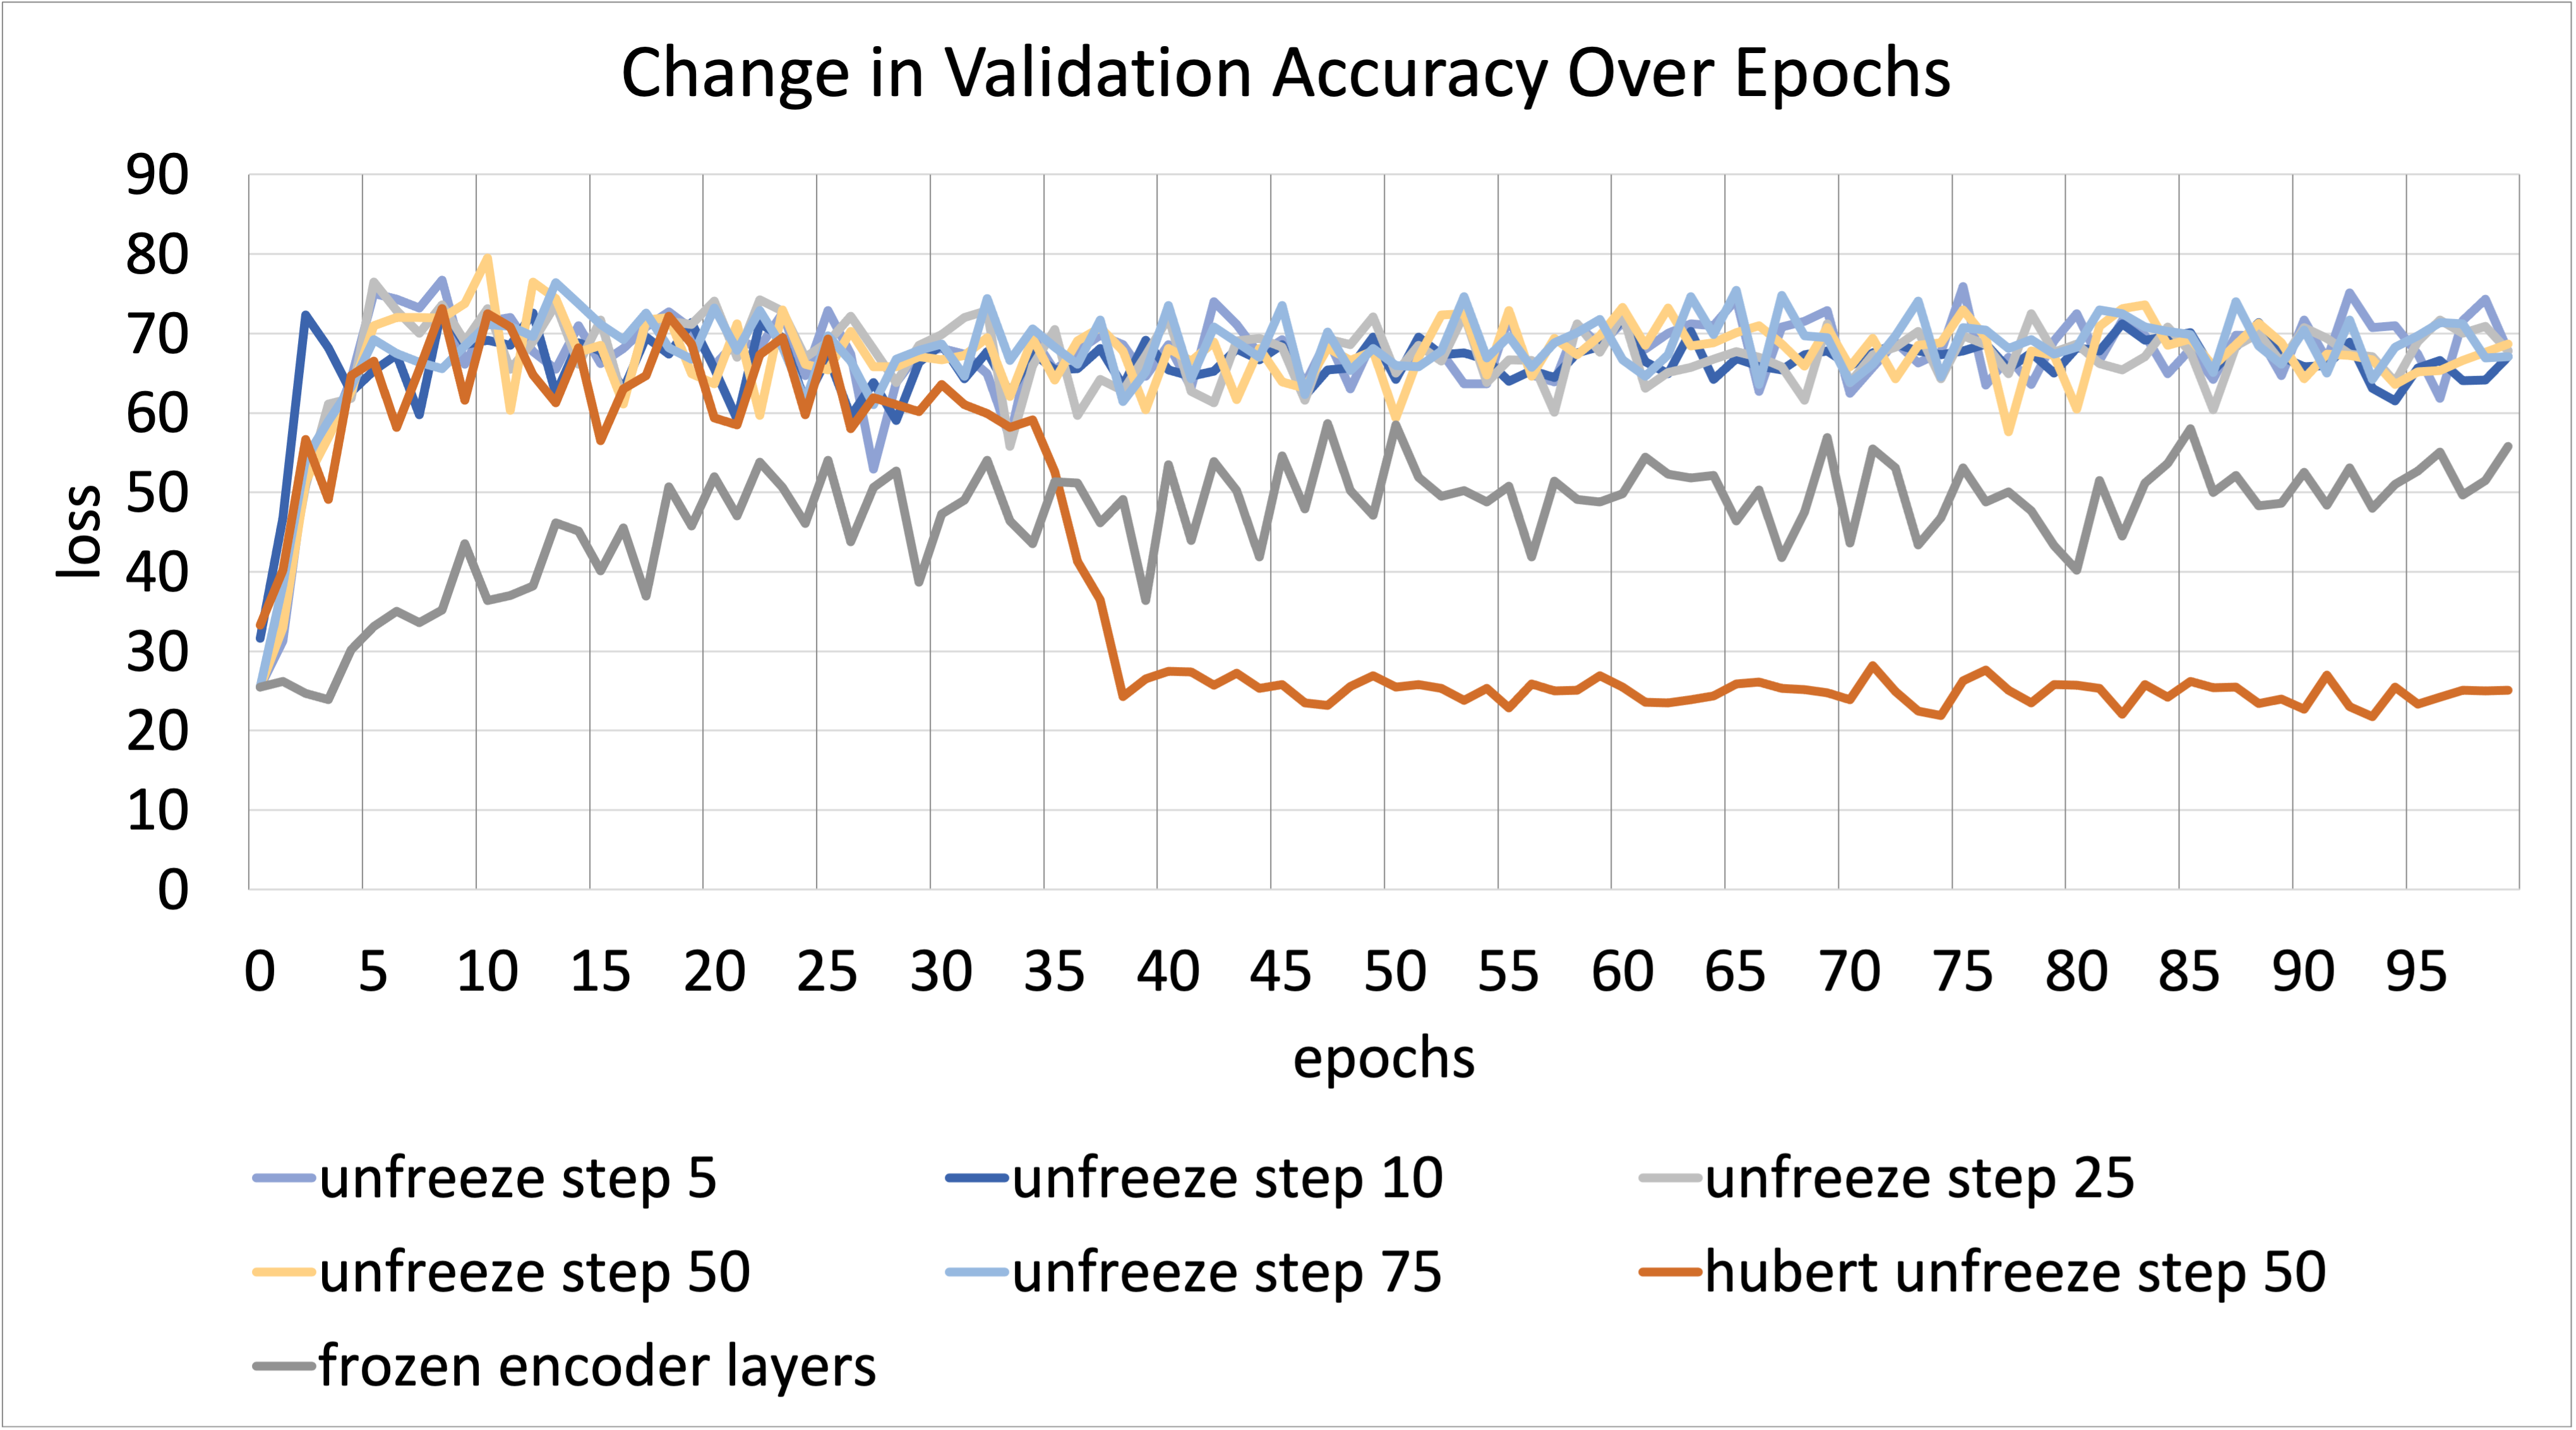
\includegraphics[width=\textwidth]{appendix/unfreezeAcc.png}
    \caption{Unfreezing encoder layers change in validation accuracy.}
\end{figure}


\begin{figure}[h!]
    \CommonHeightRow{
        \begin{floatrow}[2]
            \ffigbox[\FBwidth]
            {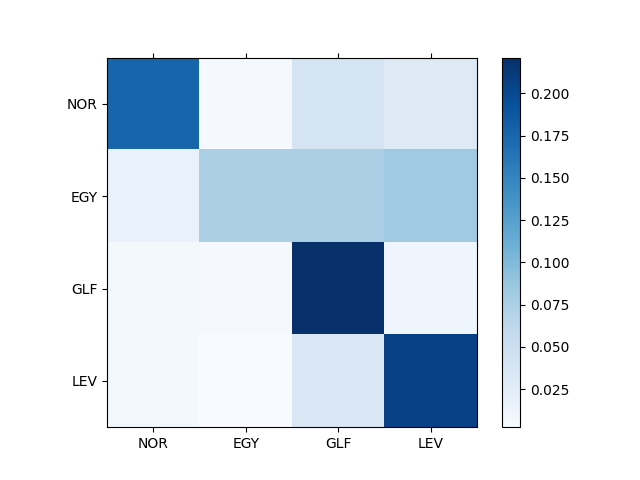
\includegraphics[height=6cm]{appendix/ADI17-xlsr-araic-unfreeze-step5-norm.png}}
            {\caption{Unfreeze step 5 \newline Normalised Confusion  Matrix Colour Map.}}
            \ffigbox[\FBwidth]
            {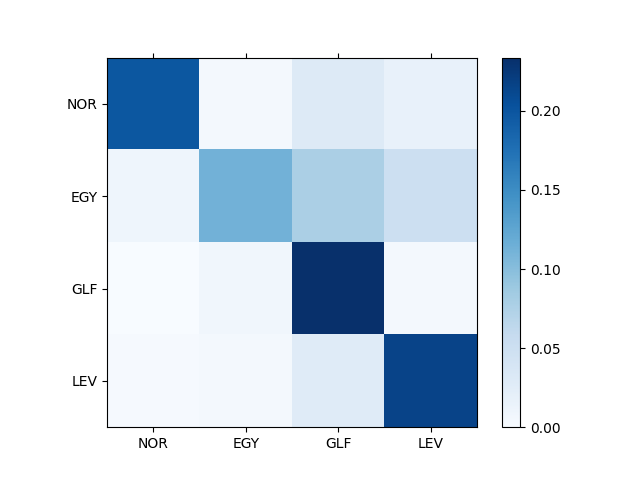
\includegraphics[height=6cm]{appendix/ADI17-xlsr-araic-unfreeze-step25-norm.png}}
            {\caption{Unfreeze step 25 \newline Normalised Confusion Matrix Colour Map.}}
        \end{floatrow}}
\end{figure}

\begin{figure}[h!]
    \CommonHeightRow{
        \begin{floatrow}[2]
            \ffigbox[\FBwidth]
            {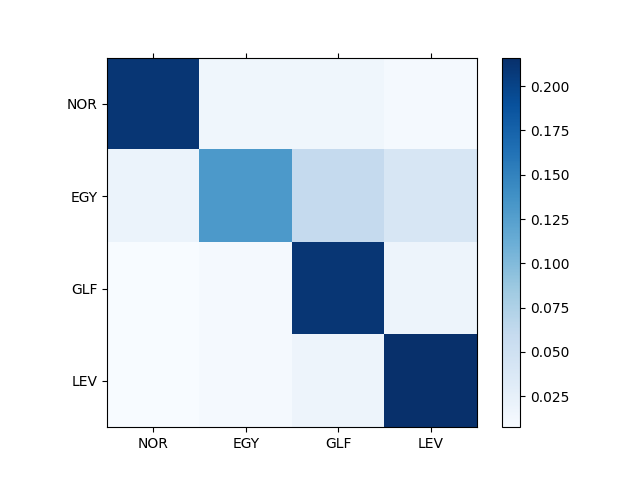
\includegraphics[height=6cm]{appendix/ADI17-xlsr-araic-unfreeze-step50-norm.png}}
            {\caption{Unfreeze step 50 \newline Normalised Confusion  Matrix Colour Map.}}
            \ffigbox[\FBwidth]
            {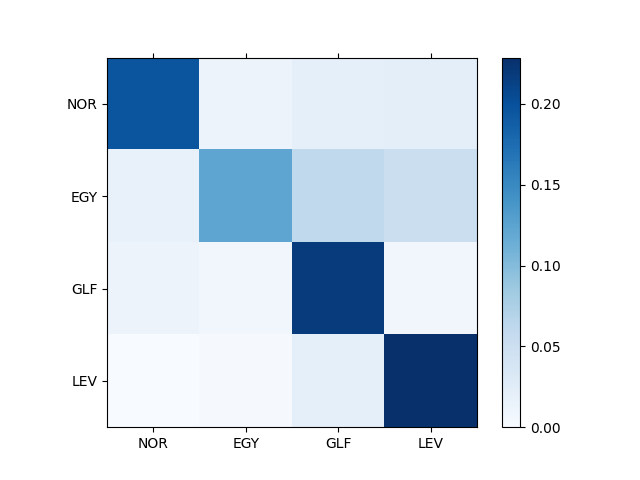
\includegraphics[height=6cm]{appendix/ADI17-xlsr-araic-unfreeze-step75-norm.png}}
            {\caption{Unfreeze step 75 \newline Normalised Confusion Matrix Colour Map.}}
        \end{floatrow}}
\end{figure}

\begin{table}
    \centering
    \caption{Classification Reports: Counteracting Bias}
    \begin{tabular}{|l|l|l|l|l|l|l|l|l|} 
    \hline
                                              & \multicolumn{4}{c|}{No Levantine}                 & \multicolumn{4}{c|}{Double Egyptian}               \\ 
    \hline
                                              & precision& recall&f1-score& support &precision&recall&f1-score&support\\ 
    \hline
    NOR                                       & 93\%          & 54\%     & 68\%         & 100     & 78\%          & 61\%     & 69\%         & 100      \\ 
    \hline
    EGY                                       & 93\%          & 54\%     & 68\%         & 100     & 85\%          & 72\%     & 78\%         & 200      \\ 
    \hline
    GLF                                       & 73\%          & 73\%     & 73\%         & 100     & 53\%          & 72\%     & 61\%         & 100      \\ 
    \hline
    LEV                                       & 61\%          & 88\%     & 72\%         & 100     & 61\%          & 71\%     & 66\%         & 100      \\ 
    \hline
    \multicolumn{1}{|r|}{accuracy}        &               &          & 71\%         & 300     &               &          & 70\%         & 500      \\ 
    \hline
    \multicolumn{1}{|r|}{macro avg}       & 76\%          & 72\%     & 71\%         & 300     & 69\%          & 69\%     & 68\%         & 500      \\ 
    \hline
    \multicolumn{1}{|r|}{weighted avg} & 76\%          & 71\%     & 71\%         & 300     & 73\%          & 70\%     & 70\%         & 500      \\
    \hline
    \end{tabular}
    \end{table}


    \begin{figure}[h!]
        \CommonHeightRow{
            \begin{floatrow}[2]
                \ffigbox[\FBwidth]
                {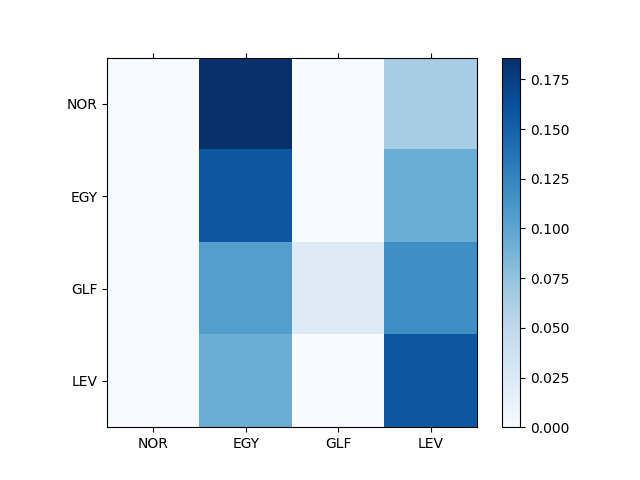
\includegraphics[height=6cm]{appendix/ADI17-xlsr-araic-25f-norm.png}}
                {\caption{25 training Files \newline Normalised Confusion Matrix Colour Map.}}
                \ffigbox[\FBwidth]
                {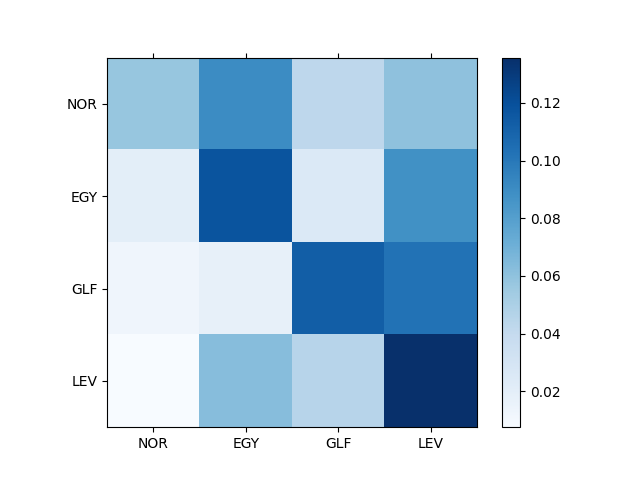
\includegraphics[height=6cm]{appendix/ADI17-xlsr-araic-50f-norm.png}}
                {\caption{50 training Files \newline Normalised Confusion Matrix Colour Map.}}
            \end{floatrow}}
    \end{figure}

    \begin{figure}[h!]
        \CommonHeightRow{
            \begin{floatrow}[2]
                \ffigbox[\FBwidth]
                {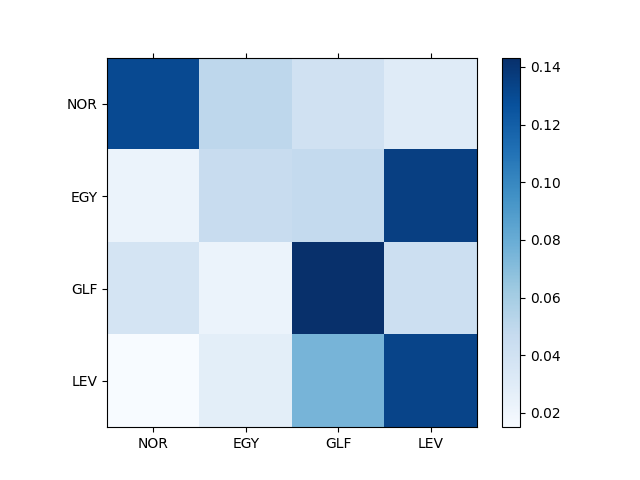
\includegraphics[height=6cm]{appendix/ADI17-xlsr-araic-100f-norm.png}}
                {\caption{100 training Files \newline Normalised Confusion  Matrix Colour Map.}}
                \ffigbox[\FBwidth]
                {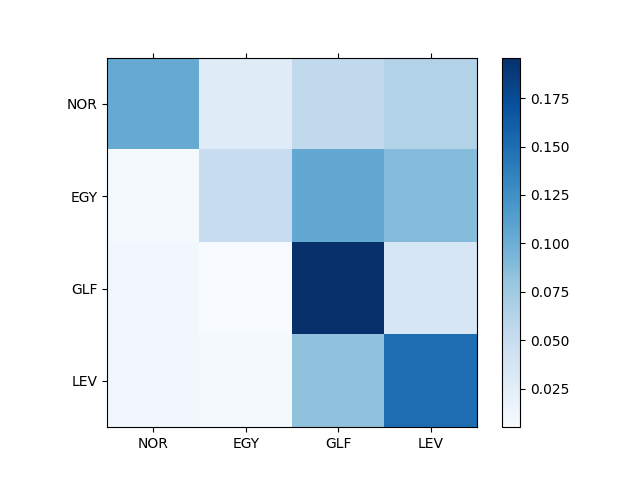
\includegraphics[height=6cm]{appendix/ADI17-xlsr-araic-200f-norm.png}}
                {\caption{200 training Files \newline Normalised Confusion Matrix Colour Map.}}
            \end{floatrow}}
    \end{figure}

    \begin{figure}[h!]
        \CommonHeightRow{
            \begin{floatrow}[2]
                \ffigbox[\FBwidth]
                {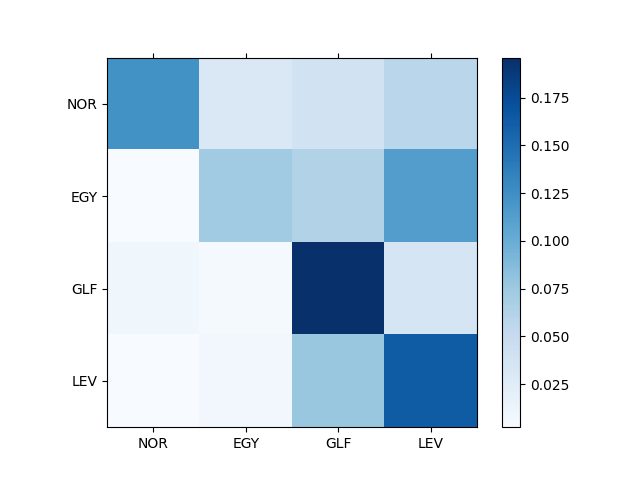
\includegraphics[height=6cm]{appendix/ADI17-xlsr-araic-400f-norm.png}}
                {\caption{400 training Files \newline Normalised Confusion  Matrix Colour Map.}}
                \ffigbox[\FBwidth]
                {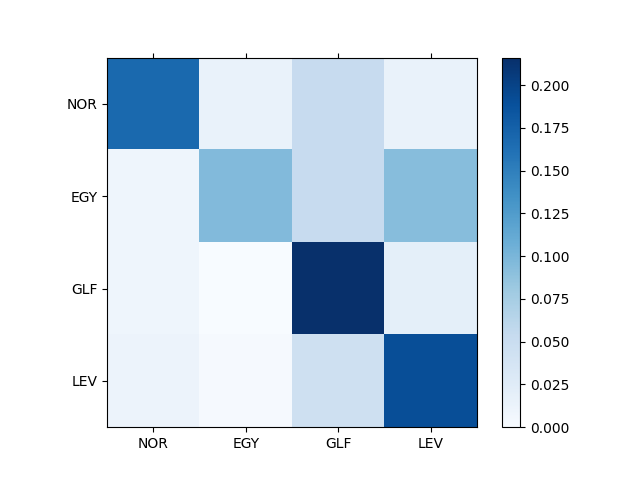
\includegraphics[height=6cm]{appendix/ADI17-xlsr-araic-600f-norm.png}}
                {\caption{600 training Files \newline Normalised Confusion Matrix Colour Map.}}
            \end{floatrow}}
    \end{figure}


    \begin{figure}[h!]
        \CommonHeightRow{
            \begin{floatrow}[2]
                \ffigbox[\FBwidth]
                {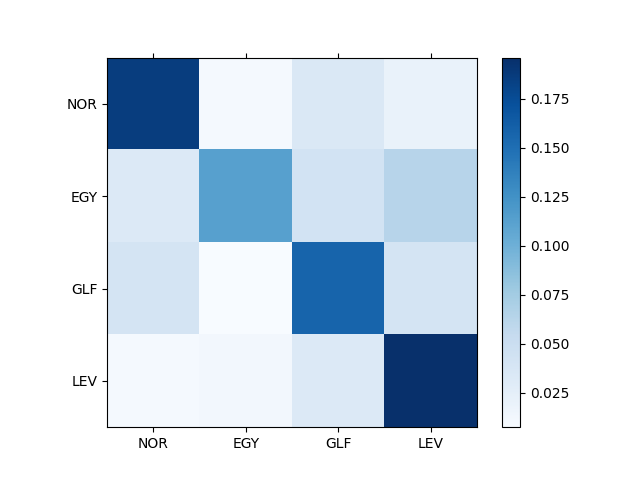
\includegraphics[height=6cm]{appendix/ADI17-xlsr-araic-800f-norm.png}}
                {\caption{800 training Files \newline Normalised Confusion  Matrix Colour Map.}}
                \ffigbox[\FBwidth]
                {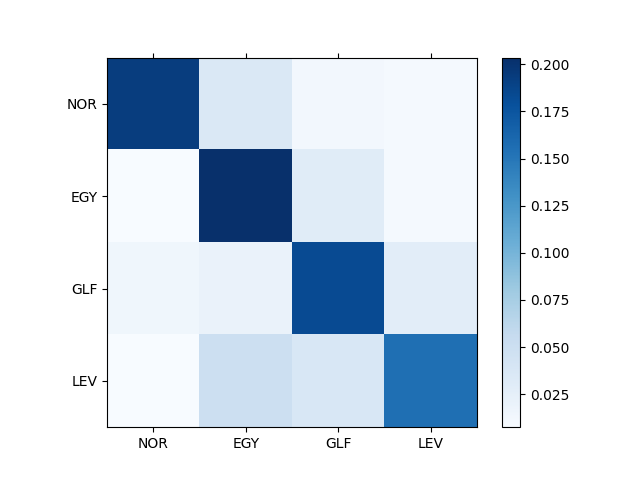
\includegraphics[height=6cm]{appendix/ADI17-xlsr-araic-1000f-norm.png}}
                {\caption{1000 training Files \newline Normalised Confusion Matrix Colour Map.}}
            \end{floatrow}}
    \end{figure}